\section{Fondamenti teorici}

\subsection{Hierarchical Model Reduction in 3D}
\begin{frame}
\tableofcontents[currentsection]
\end{frame}

 \begin{frame}
  \frametitle{Motivazione}
  \framesubtitle{esistenza di una direzione dominante}
  \begin{exampleblock}{}
 Vogliamo risolvere un certo tipo di problemi: quelli che presentano una direzione preferenziale
\begin{center}
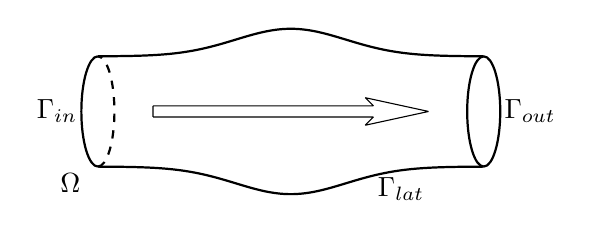
\begin{tikzpicture}
[scale=0.7]
\def\xi{0};
\def\xo{7};
\def\c{3.5};
\def\r{1};
\def\sig{2};
\def\rmax{0.5};
\def\rtot{\rmax+\r};
\def\yd{-0.1}
\def\yu{-\yd}
\def\xs{1}
\def\xf{5}
\def\xe{6}
\def\xa{0.15}
\def\ya{0.15}
 \draw (\xs,\yd) -- (\xf,\yd)
       (\xf,\yd) -- (\xf-\xa,\yd-\ya)
       (\xf-\xa,\yd-\ya) -- (\xe,0)
       (\xe,0) -- (\xf-\xa,\yu + \ya)
       (\xf-\xa,\yu + \ya) -- (\xf,\yu)
       (\xf,\yu) -- (\xs,\yu)
       (\xs,\yu) -- (\xs,\yd);
\draw[thick] (\xi,\r) arc (90:270:0.3cm and \r cm);
\draw[dashed,thick] (\xi,-\r) arc (-90:90:0.3cm and \r cm);

\draw[thick] (\xo,\r) arc (90:270:0.3cm and \r cm);
\draw[thick] (\xo,-\r) arc (-90:90:0.3cm and \r cm);

\draw[thick,parametric,domain=-\xi:\xo,samples=200,variable=\t] plot ({\t},{\r+\rmax*exp{-pow(\t-\c,2)/\sig}});
\draw[thick,parametric,domain=-\xi:\xo,samples=200,variable=\t] plot ({\t},{-\r-\rmax*exp{-pow(\t-\c,2)/\sig}});
\def\po{0.9};
\node[left] at(\xi-0.2,0) {$\Gamma_{in}$};
\node[right] at(\xo +0.2,0) {$\Gamma_{out}$};
\node at (\xi -0.5,-1.3) {$\Omega$};
\node at (\c +2,-\r-0.4) {$\Gamma_{lat}$};
\end{tikzpicture}
\end{center}
\end{exampleblock}
\begin{center}
\tikzstyle{3d} = [ellipse, draw, fill=red!50, 
    text width=7em,text badly centered, inner sep=0pt]

\tikzstyle{1d} = [ellipse, draw, fill=blue!30, 
    text width=7em,text badly centered, inner sep=0pt]
    
\tikzstyle{himod} = [rectangle, draw, fill=blue!50!red!50!white]
\begin{tikzpicture}
\def\x{7};
\node[1d] (1d) at (0,0) {\textbf{Modello 1D}\\{\footnotesize Bassa precisione}\\{\footnotesize Economico}};
\node[3d] (3d) at (\x,0) {\textbf{Modello 3D}\\{\footnotesize Alta precisione}\\{\footnotesize Costoso}};
\node[himod] (himod) at (\x/2,0) {HiMod};
\path[draw,thick,dashed,->] (1d) -- (himod);
\path[draw,thick,dashed,<-] (himod) -- (3d);

			  
%smily face sinistra
\def\f{1.0}
\def\alt{-0.5}
\def\rad{0.15}
\draw[thin] (\f,\alt) circle(\rad cm);
\draw[thin] plot [smooth,tension=1.5] coordinates{(\f - 0.5*\rad,\alt - 0.4*\rad) (\f + 0*\rad,\alt - 0.7*\rad) (\f + 0.5*\rad,\alt -0.4*\rad)};
% \draw[thin, fill=black] (\f+0*\rad,\alt-0.2*\rad) circle (0.1*\rad);
\draw[thin] plot [smooth,tension=1.5] coordinates{(\f-0.4*\rad,\alt+0.4*\rad) (\f-0.3*\rad,\alt +0.5*\rad) (\f-0.2*\rad,\alt+0.4*\rad)};
\draw[thin] plot [smooth,tension=1.5] coordinates{(\f+0.4*\rad,\alt+0.4*\rad) (\f+0.3*\rad,\alt+0.5*\rad) (\f+0.2*\rad,\alt+0.4*\rad)};

  
%smily face sinistra
\def\f{8.25}
\def\alt{-0.05}
\def\rad{0.15}
\draw[thin] (\f,\alt) circle(\rad cm);
\draw[thin] plot [smooth,tension=1.5] coordinates{(\f - 0.5*\rad,\alt - 0.4*\rad) (\f + 0*\rad,\alt - 0.7*\rad) (\f + 0.5*\rad,\alt -0.4*\rad)};
% \draw[thin, fill=black] (\f+0*\rad,\alt-0.2*\rad) circle (0.1*\rad);
\draw[thin] plot [smooth,tension=1.5] coordinates{(\f-0.4*\rad,\alt+0.4*\rad) (\f-0.3*\rad,\alt +0.5*\rad) (\f-0.2*\rad,\alt+0.4*\rad)};
\draw[thin] plot [smooth,tension=1.5] coordinates{(\f+0.4*\rad,\alt+0.4*\rad) (\f+0.3*\rad,\alt+0.5*\rad) (\f+0.2*\rad,\alt+0.4*\rad)};

  
%sad face destra
\def\f{7.8}
\def\alt{-0.5}
\def\rad{0.15}
\draw[thin] (\f,\alt) circle(\rad cm);
\draw[thin] plot [smooth,tension=1.5] coordinates{(\f-0.3*\rad,\alt-0.6*\rad) (\f-0.2*\rad,\alt-0.5*\rad) (\f +0.3*\rad,\alt-0.5*\rad)};
\draw[thin] (\f-0.4*\rad,\alt+0.4*\rad) -- (\f-0.2*\rad,\alt +0.3*\rad);
\draw[thin] (\f+0.4*\rad,\alt+0.5*\rad) -- (\f+0.2*\rad,\alt +0.4*\rad);
% \draw[thin, fill=black] (\f+0*\rad,\alt-0.2*\rad) circle (0.1*\rad);
%sad face sinistra
\def\f{1.4}
\def\alt{-0.05}
\def\rad{0.15}
\draw[thin] (\f,\alt) circle(\rad cm);
\draw[thin] plot [smooth,tension=1.5] coordinates{(\f-0.3*\rad,\alt-0.6*\rad) (\f-0.2*\rad,\alt-0.5*\rad) (\f +0.3*\rad,\alt-0.5*\rad)};
\draw[thin] (\f-0.4*\rad,\alt+0.4*\rad) -- (\f-0.2*\rad,\alt +0.3*\rad);
\draw[thin] (\f+0.4*\rad,\alt+0.5*\rad) -- (\f+0.2*\rad,\alt +0.4*\rad);
% \draw[thin, fill=black] (\f+0*\rad,\alt-0.2*\rad) circle (0.1*\rad);
\end{tikzpicture}
\end{center}
 \end{frame}

 \begin{frame}
 \frametitle{Impostazione geometrica}
 \framesubtitle{il dominio}
 
\begin{itemize}
 \item Fibra di supporto rettilinea \textcolor{blue}{$\Omega_{1D}$} dove avviene la dinamica dominante.
 \item Suddivisione del dominio in slices \textcolor{red}{$\gamma_x$} ortogonali alla fibra di supporto.
\end{itemize}

$$\Omega=\bigcup_{x\in\Omega_{1D}}\gamma_x$$
\begin{center}
\begin{tikzpicture}
[scale=0.8]
\def\xi{0};
\def\xo{7};
\def\c{3.5};
\def\r{1};
\def\sig{2};
\def\rmax{0.5};
\def\rtot{\rmax+\r};

\draw[thick] (\xi,0) arc (90:270:0.3cm and \r cm);
\draw[dashed,thick] (\xi,-2*\r) arc (-90:90:0.3cm and \r cm);

\draw[thick] (\xo,0) arc (90:270:0.3cm and \r cm);
\draw[thick] (\xo,-2*\r) arc (-90:90:0.3cm and \r cm);

% \draw[->] (-2,0) -- (2,0);
% \draw[->] (0,-2) -- (0,2);
\draw[thick,parametric,domain=-\xi:\xo,samples=200,variable=\t] plot ({\t},{\rmax*exp{-pow(\t-\c,2)/\sig}});
\draw[thick,parametric,domain=-\xi:\xo,samples=200,variable=\t] plot ({\t},{-2*\r-\rmax*exp{-pow(\t-\c,2)/\sig}});
\draw[thick,parametric,domain=-\xi:\xo,samples=200,variable=\t,dashed,blue] plot ({\t},{-\r});
\draw[color=red!70,pattern=north west lines, pattern color=red!20, thick] (\c,-\r) ellipse (0.3 and \rtot);
\def\po{0.9};
\node[below,blue] at (\xo*\po,-\r) {$\Omega_{1D}$};
\node[below,red] at (\c,-2*\r-\rmax) {$\gamma_x$};
\node[left] at(\xi-0.2,-\r) {$\Gamma_{in}$};
\node[right] at(\xo +0.2,-\r) {$\Gamma_{out}$};
\node at (\xi -0.5,-\r-1.3) {$\Omega$};
\node at (\c +2,-2*\r-0.4) {$\Gamma_{lat}$};
\end{tikzpicture}
\end{center}
\end{frame}

 \begin{frame}
 \frametitle{Idea}
 \framesubtitle{mapping e serie di Fourier}
 \begin{itemize}
  \item mappare $\Omega$ in un dominio di riferimento $\widehat \Omega$ in modo che $$\hat \gamma_{\hat x}=\hat \gamma\,\,\forall \hat x\in\widehat\Omega_{1D}$$
  \item espandere, in direzione trasversale, la soluzione rispetto alla base di Fourier generalizzata $$\{\varphi_k(\yhat,\zhat)\}_{k\in\mathbb{N}}$$
 \end{itemize}
 \textcolor{red}{\footnotesize\textbf{Notazione}}{\footnotesize: lavoreremo gi\`a sul riferimento, non useremo quindi i cappelli.}
 \begin{block}{Spazi in direzione trasversale}
 \footnotesize
  $$V^\infty_\gamma=\left\{v(y,z)=\sum_{k=1}^\infty v_k\varphi_k(y,z)\right\}$$
  $$V^m_\gamma=\left\{v(y,z)=\sum_{k=1}^m v_k\varphi_k(y,z)\right\}$$
 \end{block}
 \end{frame}
\begin{frame}
 \frametitle{Processo di riduzione}
 \framesubtitle{Spazi ridotti}
 Usiamo uno spazio $V_{1D}$ di tipo $H^1(\Omega_{1D})$ lungo la \textbf{direzione principale}.
 
 Possiamo ora definire gli spazi ridotti come \textbf{spazi prodotto}
 \begin{exampleblock}{Spazi ridotti}
 {\footnotesize
  $$V^\infty(\Omega)=V_{1D}\otimes V^\infty_\gamma:=\left\{v(x,y,z)=\sum_{k=1}^\infty v_k(x)\varphi_k(y,z), v_k\in V_{1D}\right\}.$$
  $$V^m(\Omega)=V_{1D}\otimes V^m_\gamma:=\left\{v(x,y,z)=\sum_{k=1}^m v_k(x)\varphi_k(y,z), v_k\in V_{1D}\right\}.$$
  }
  
  \`E lo spazio delle \textbf{combinazioni lineari a coefficienti in} $\mathbf{V_{1D}}$ delle funzioni di base della fibra trasversale.
  \end{exampleblock}
\end{frame}

\begin{frame}
 \frametitle{Il problema}
 \framesubtitle{Caso condizioni di Dirichlet}
 Il \textbf{problema} che vogliamo risolvere ...
 \begin{exampleblock}{}
 \begin{equation}
  \begin{cases}
   -\mu\Delta u + \vect{\beta}\cdot \nabla u +\sigma u = f\text{ in }\Omega\\
   u=0\text{ su }\partial{\Omega}
  \end{cases}
 \end{equation}
 \end{exampleblock}
 ... e la sua \textbf{formulazione debole}
 \begin{exampleblock}{}
 \noindent{Trovare $u\in H^1_0(\Omega)$ tale che}
 \begin{equation}
  \int_{\Omega} \mu\nabla u \nabla v +\vect{\beta}\cdot \nabla uv + \sigma uv d\Omega=\int_{\Omega}fv d\Omega\qquad\forall v \in H^1_0(\Omega).
 \end{equation}
 \end{exampleblock}


\end{frame}

 \begin{frame}
  \frametitle{Modelli ridotti}
  \framesubtitle{Problemi 1D accoppiati}
 \begin{center}
  \tikzstyle{ellisse} = [ellipse, draw, fill=blue!30, 
    text width=7em,text badly centered, inner sep=0pt]
  \tikzstyle{cerchio} = [circle, draw, fill=green!30, 
    text width=2em,text badly centered, inner sep=0pt]
   \tikzstyle{rec} = [rectangle, draw, fill=green!50]
    \begin{tikzpicture}
    \footnotesize
     \node[ellisse] (3D) at (0,0) {\footnotesize \textbf{Problema 3D} in forma debole su $\mathbf{V^m(\Omega)}$};
     \node[rec] (int) at (4,0) {\footnotesize Integrazione su $\boldsymbol{\gamma}$};
     \node[ellisse] (1Dcoupled) at (8,0) {\footnotesize $\mathbf{m}$ \textbf{problemi 1D} in forma debole su $\mathbf{V_{1D}}$};
     \node[cerchio] (r) at (5.5,-1) {$r^{st}_{k,j}$};
     \draw[->] (3D) -- (int);
     \draw[->] (int)-- (1Dcoupled);
    \draw plot[smooth,tension=1.3] coordinates{(4,-0.5) (4.2,-1) (5.15,-1)};
    \draw (4.95,-0.95)--(5.13,-1);
    \draw (5.,-1.15)--(5.13,-1);
    \end{tikzpicture}
 \end{center}
  I coefficienti $r^{st}_{k,j}$ accoppiano i problemi 1D: comprimono le informazioni nella fibra trasversale 
  tramite opportuni integrali su $\gamma$.
 \begin{exampleblock}{}
Trovare $\{u_k\}_{k=1}^m$ con $u_k\in V_{1D}\,\,\forall k=1\ldots m$ tale che
  {\footnotesize
\begin{equation}
\label{eq:modalreducedcoeff}
 \sum_{k=1}^m\int_{\Omega_{1D}}
 \biggl[
 \underbrace{\hat r^{11}_{k,j}\dpar{ u_k}{x}\dpar{\theta_j}{x}}_{\textbf{Diffusione}}
+\underbrace{\hat r^{10}_{k,j}\dpar{ u_k}{x}\theta_j}_{\textbf{Trasporto}}
+\underbrace{\hat r^{00}_{k,j} u_k\theta_j}_{\textbf{Reazione}}
dx\biggr]=\int_{\Omega_{1D}}\nsp{2}\underbrace{\theta_jf_k}_{\textbf{Forzante}} dx. \psp{3}\forall j=1\ldots m\quad\theta_j\in V_{1D} 
\end{equation}}
\end{exampleblock}
 \end{frame}
 \begin{frame}
  \frametitle{Struttura alegebrica}
  \framesubtitle{Pattern di sparsit\`a}
  Per $V_{1D}$ utilizziamo una discretizzazione elementi finiti P1 ottenendo il seguende 
  \textbf{pattern di 
  sparsit\`a}.
  
  \begin{figure}
   \centering
  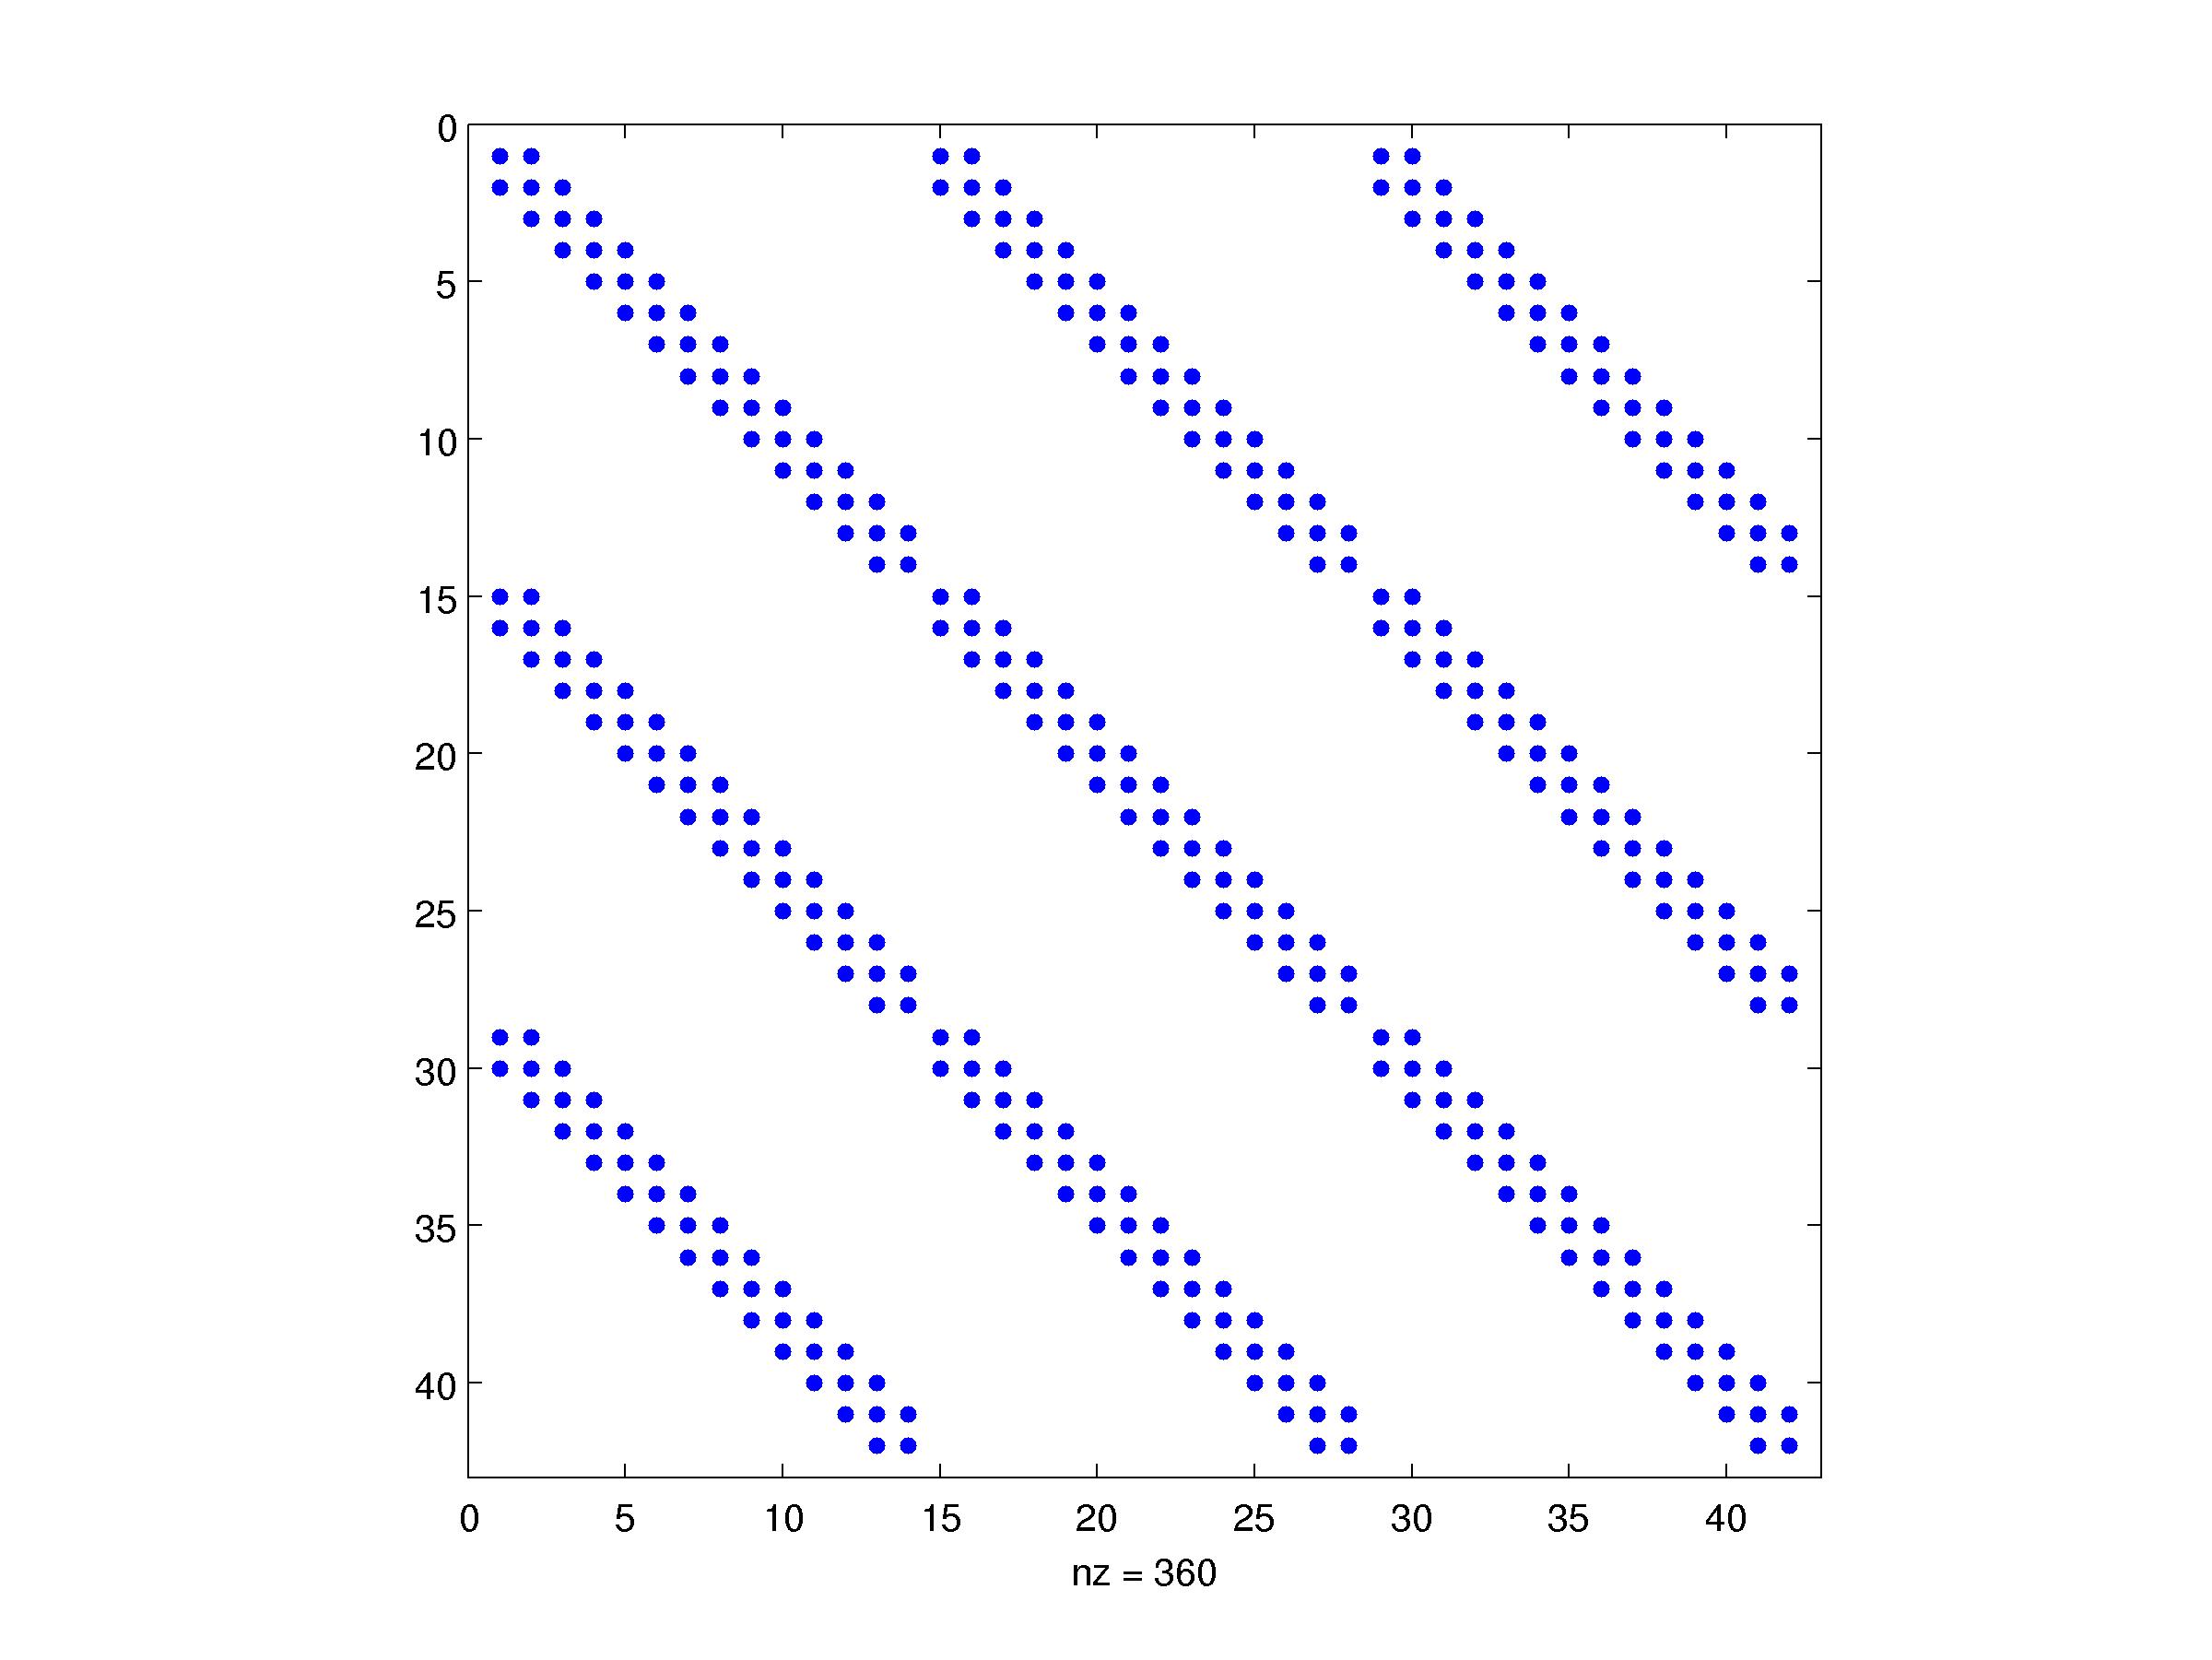
\includegraphics[scale=0.35,trim=4.2cm 1.5cm 3.5cm 1cm, clip=true]{Varie/spy_14elem3modes}
 
  \end{figure}
  \begin{center} 14 elementi, 3 modi.\end{center}
  
  \textbf{\red{Nota:}} i blocchi si riferiscono alle \red{frequenze}, ogni blocco ha il pattern proprio degli \red{elementi finiti}
 \end{frame}

\begin{frame}
 \frametitle{Scelta della base}
 \framesubtitle{Basi trigonometriche e polinomi di Legendre}
 In \textbf{letteratura} \`e stato considerato il problema di \textbf{Dirichlet} in \textbf{2D}.
 Le basi scelte sono state
 \begin{columns}
 \begin{column}{0.7\textwidth}
 \begin{itemize}
  \item Funzioni \textcolor{red}{trigonometriche}: $\sin(\pi k x)\text{ in }(0,1)$ 
  \item Polinomi di \textcolor{red}{Legendre} moltiplicati per un \\fattore $(1-x^2)$ + Gram-Schmidt 
 \end{itemize}
 \end{column}
 \begin{column}{0.3\textwidth}
 \footnotesize
  [Prof. Perotto]
  \vspace{0.45cm}
  
  \noindent[Prof. Blanco, LNCC]
 \end{column}
 \end{columns}
\begin{alertblock}{In questo progetto}
 abbiamo esteso l'approccio \textbf{trigonometrico} al \textbf{caso 3D} con condizioni al bordo omogenee di tipo pi\'u \textbf{generale}.
\end{alertblock}

\end{frame}

 
\subsection{Basi istruite}

\begin{frame}
\tableofcontents[currentsection]
\end{frame}

\begin{frame}
 \frametitle{Ipotesi geometriche}
 \framesubtitle{Dominio parallelepipedo}
 \begin{center}
\begin{tikzpicture}
[scale=1.5]

\draw [thick] (2,0) rectangle (3,1);
\node[red] at (+0.25,1.35) {$\Gamma_{in}$};
\node[red] at (2.75,0.75) {$\Gamma_{out}$};
\node[red] at (1.95,1.32) {$\Gamma_{lat}$};
\node[green!90!blue] at (1.1,0.6) {$\boldsymbol\gamma$};
% \node at (0.7,0.88) {$\gamma}$};
\node[blue!90!red] at (3.5,-0.2) {$\Omega_{1D}$};


\draw [thick] (2,1)--(0,2)--(1,2)--(3,1);
\draw [thick] (2,0)--(0,1)--(0,2);

%dim.
\draw [<->,thin] (-0.1,0.95) -- (1.85,-0.05);
\node [left] at (1.05,0.3) {\footnotesize$L_x$};

\draw [<->,thin] (2.05,-0.1) -- (3.1,-0.1);
\node [below] at (2.7,-0.08) {\footnotesize$L_y$};


\draw [<->,thin] (-0.1,1) -- (-0.1,2);
\node [left] at (-0.08,1.55) {\footnotesize$L_z$};

\draw [dashed,thick] (0,1)--(1,1)--(1,2);
\draw [dashed,thick] (1,1)--(3,0);

\draw [color=green!75!blue,pattern=north west lines, pattern color=green!75!blue, thick] (0.5,0.75) rectangle (1.5,1.75);

\draw [thick,dashed, ->,blue!90!red] (-0.5,2)--(3.5,0);

\def\x{-1};
\def\y{0.8};

\def\l{0.3};
%assi
\draw[->,thin] (\x,\y) -- (\x +\l,\y);
\draw[->,thin] (\x,\y) -- (\x,\y+\l);
\draw[->,thin] (\x,\y) -- (\x +\l,\y-\l +0.17);
\node[right] at (\x +\l,\y) {\footnotesize $y$};
\node[left] at (\x,\y+\l) {\footnotesize $z$};
\node[below] at (\x +\l,\y-\l +0.17) {\footnotesize $x$};
\end{tikzpicture}
\end{center}
\textbf{Ipotesi} per le condizioni al bordo su $\textcolor{red}{\Gamma_{lat}}$
\begin{itemize}
 \item \textbf{omogenee}
  \item di ogni tipo ma con \textbf{coefficienti costanti}
\end{itemize}
\end{frame}

\begin{frame}
  \frametitle{Base teorica}
  \framesubtitle{Teorema spettrale per forme bilineari}
  \begin{block}{}
Sia V uno spazio di tipo $H^1$.
Sia $a(\cdot,\cdot)$ una \textbf{forma bilineare} in V, continua, \textbf{simmetrica} e debolmente coerciva 
{\footnotesize $(a(u,u)\geq \alpha||u||_V^2+\lambda_0||u||^2_{L^2} )$}. Allora:
\begin{itemize}
\item[(a)] L'insieme degli autovalori \`e numerabile ed \`e una successione $\{\lambda_m \}_{m\geq 1}$ tale che  $\lambda_m\rightarrow +\infty$;
\item[(b)] se u ,v sono autofunzioni corrispondenti ad autovalori differenti, allora $$a(u,v) = 0 = (u,v)_{L^2}.$$
Inoltre, $L^2$ ha una base ortonormale $\{ u_m \}_{m\geq 1}$ di autofunzioni di a;
\item[(c)] la successione $\{u_m / \sqrt{\lambda_0+\lambda_m} \}_{m\geq 1}$ \`e anche una base ortonormale in V, rispetto al prodotto scalare
\begin{displaymath}
((u,v))=a(u,v)+\lambda_0 (u,v)_{L^2}.
\end{displaymath}
\end{itemize}
\end{block}
\end{frame}

\begin{frame}
 \frametitle{Problema agli autovalori ausiliario}
 \framesubtitle{Due sottoproblemi agli autovalori}
 \textbf{Problema agli autovalori su} $\boldsymbol\gamma$: un caso con condizioni al bordo miste Dirichlet e Robin
 \begin{columns}
  \begin{column}{0.6\textwidth}
\begin{equation}
    \begin{cases}
     -\Delta u = \lambda u &\text{ in }\gamma\\
     u=0 &\text{ su } 1,3,4\\
     \mu \dpar{u}{y} + \chi u = 0 &\text{ su } 2\\
    \end{cases}
 \end{equation}
  \end{column}
  \begin{column}{0.3\textwidth}
   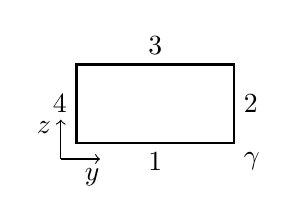
\begin{tikzpicture}
    \draw[thick] (0,0) rectangle (2,1);
    \node[left] at (0,0.5){$4$};
    \node[below] at (1,0){$1$};
    \node[right] at (2,0.5){$2$};
    \node[above] at (1,1){$3$};
    \node[below right] at (2,0) {$\gamma$};
    
    \draw[thin,->] (-0.2,-0.2) -- (0.3,-0.2);
    \draw[thin,->] (-0.2,-0.2) -- (-0.2,0.3);
    \node[left] at  (-0.2,0.2){$z$};
    \node[below] at (0.2,-0.2) {$y$};
    
    \end{tikzpicture}

  \end{column}
 \end{columns}
 \textbf{Ipotesi:} $u(y,z)=Y(y)Z(z)$
 {\footnotesize
 \begin{equation}
 \begin{cases}
  -\frac{Y''}{Y}-\frac{Z''}{Z} = \lambda&\longrightarrow \red{-Y''=K_yY},\psp{2} \blue{-Z''= K_zZ},\psp{2}\lambda=K_z+K_y\\
  u=0 \text{ su }1,3&\longrightarrow Y(y)\blue{Z(1)=0},\psp{1} Y(y)\blue{Z(0)=0} \psp{3}\forall y\in(0,L_y)\\
  u=0 \text{ su }4&\longrightarrow \red{Y(0)}Z(z)\red{=0} \psp{3}\forall z\in(0,L_z)\\
  \mu \dpar{u}{y} + \chi u = 0 \text{ su } 2&\longrightarrow \red{\mu \dpar{Y}{y}(1)}Z(z) + \red{\chi Y(1)}Z(z)\red{ = 0} \psp{3}\forall z\in(0,L_z)\\
  \end{cases}
 \end{equation}}
 \end{frame}
 
 \begin{frame}
 \frametitle{Soluzione (semi-)analitica del problema agli autovalori}
 \framesubtitle{Soluzione dei due sottoproblemi e combinazione dei risultati}
 \begin{columns}
 \footnotesize
  \begin{column}{0.5\textwidth}
  \begin{equation}
  \begin{cases}
   -Y''=K_yY \text{ in }(0,L_y)\\
   Y(0)=0\\
   \mu Y'(L_y)+\chi Y(L_y)=0\\
  \end{cases}
 \end{equation}
 \end{column}
  \begin{column}{0.5\textwidth}
      \begin{equation}
  \begin{cases}
   -Z''= K_zZ\text{ in }(0,L_z)\\
   Z(0)=0\\
   Z(L_z)=0\\   
  \end{cases}
 \end{equation}
\end{column}
\end{columns}

\begin{alertblock}{}
  $$\Longrightarrow\{\varphi_{y,p}(y),K_{y,p}\}_{p=1}^\infty\psp{38}\Longrightarrow\{\varphi_{z,q}(z),K_{z,q}\}_{q=1}^\infty$$
\end{alertblock}

\textbf{Combinando} queste successioni otteniamo le 
 soluzioni del \textbf{problema iniziale} agli autovalori su $\gamma$
 \begin{alertblock}{}
 \begin{equation}
  \{\varphi_k(y,z),\lambda_k\}=\{\varphi_{y,p}(y)\varphi_{z,q}(z),K_{y,p}+K_{z,q}\}
 \end{equation}
 \end{alertblock}
 Due questioni da affrontare...
 \begin{itemize}
  \item Come risolvere il singolo problema agli autovalori \textbf{?}
  \item Siamo interessati ad ordinare le $\{\varphi_k(y,z)\}$ rispetto al valore di $\{\lambda_k\}$: come \`e possibile farlo
a partire da $\{K_{y,p}\}$ e $\{K_{z,q}\}$ \textbf{?}
 \end{itemize}
 \end{frame}
\begin{frame}
 \frametitle{Risoluzione sottoproblema agli autovalori}
 \framesubtitle{Ricerca degli zeri}
 Forma della soluzione generale
 \begin{alertblock}{}
 \begin{equation}
  \phi_{y,k}(y)=A_ksin(w_{y,k}y)+B_kcos(w_{y,k}y), \psp{3}w_{y,k}^2=K_{y,k}
 \end{equation}
 \end{alertblock}
 \begin{center}
 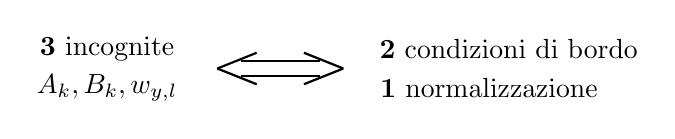
\begin{tikzpicture}
  \node at (2.3,0.25) {\textbf{3} incognite};
  \node at (2.3,-0.25) {$A_k,B_k,w_{y,l}$};
  \draw[thick] (4,0.1)--(5,0.1);
 \draw[thick] (4,-0.1)--(5,-0.1);
 \draw[thick] (3.7,0) -- (4.2,0.2);
 \draw[thick] (3.7,0) -- (4.2,-0.2);
 \draw[thick] (5.3,0) -- (4.8,0.2);
 \draw[thick] (5.3,0) -- (4.8,-0.2);
 \node at (7.4,0.25) {\textbf{2} condizioni di bordo};
 \node at (7.15,-0.25) {\textbf{1} normalizzazione};
 \end{tikzpicture}
 \end{center}
\red{\textbf{Note:}} \red{1.} ortogonalit\`a garantita dal teorema spettrale\\
$\psp{18}$\red{2.} equazione spesso non lineare in $w_{y,k}$

%{\footnotesize
%\begin{tabular}{l l l l l l l l }
%\toprule
%a	&b	&c		&d	&Type			&$\lambda_k$ 					 	&A&B\\
%\midrule
%$\chi$&$\mu$	&$\chi$	&$\mu$	&Rob-Rob		&$\tan{(\sqrt{\lambda_k})}
%(\chi-\frac{\mu^2\lambda_k}{\chi})+2\mu\sqrt{\lambda_k}=0$								&1&$\frac{\mu\sqrt{\lambda_k}}{\chi}$\\
%1	&0	&$\chi$	&$\mu$	&Dir-Rob	&$\tan{(\sqrt{\lambda_k})}+\frac{\mu\sqrt{\lambda_k}}{\chi}=0$	&1&$-\tan{(\sqrt{\lambda_k})}$  \\
%1	&0	&1		&0	&Dir-Dir	&$\lambda_k=(k\pi)^2$						&1&0\\
%0	&1	&0		&1	&Neu-Neu	&$\lambda_k=(k\pi)^2$						&0&1\\
%
%\bottomrule
%\end{tabular}}
\end{frame}


\begin{frame}
 \frametitle{Un problema di ordinamento}
 \framesubtitle{Esempio caso condizioni di Dirichlet}
 \textbf{Esempio:} condizioni di Dirichlet su $\Gamma_{lat}$ con $L_y=\pi$ e $L_z=3\pi/2$.
 
 Si ha che
 \begin{alertblock}{}
 \begin{equation}
  K_{y,p}=p^2, K_{z,q}=(2/3q)^2.
 \end{equation} 
 \end{alertblock}
 \vspace{0.5cm}
 
 {\footnotesize
 \begin{tabular}{c|lc|lc|lc|lc|lc|lc}
  \blue{$K_{y,p}$}&1&p=1&4&p=2&9&p=3&1&p=1&4&p=2&...\\%9&p=3\\%&1 p=1&4 p=2&9 p=3\\
  \blue{$K_{z,q}$}&4/9&q=1&4/9&q=1&4/9&q=1&16/9&q=2&16/9&q=2&...\\%16/9&q=2\\%&81/4 q=3&81/4 q=3&81/4 q=3\\
  \midrule
  \blue{$\lambda_k$}&1.44&k=1&4.44&k=3 &9.44&k=5&2.77&k=2&5.77&k=4&...\\%10.77&k=6 \\%&21.25&24.25&29.25\\
\end{tabular}}
 \vspace{0.5cm}

Per  il problema dell'ordinamento abbiamo sviluppato l'algoritmo implementato in \red{\texttt{EigensProvider}}.
\end{frame}